% Auto-generated paper review summary (Kelly)
\documentclass{article}
\usepackage[margin=1in]{geometry}
\usepackage{graphicx}
\usepackage{hyperref}

\begin{document}

\section*{InterFormer: Effective Heterogeneous Interaction Learning for Click-Through Rate Prediction (2025)}

\begin{figure}[h]
  \centering
  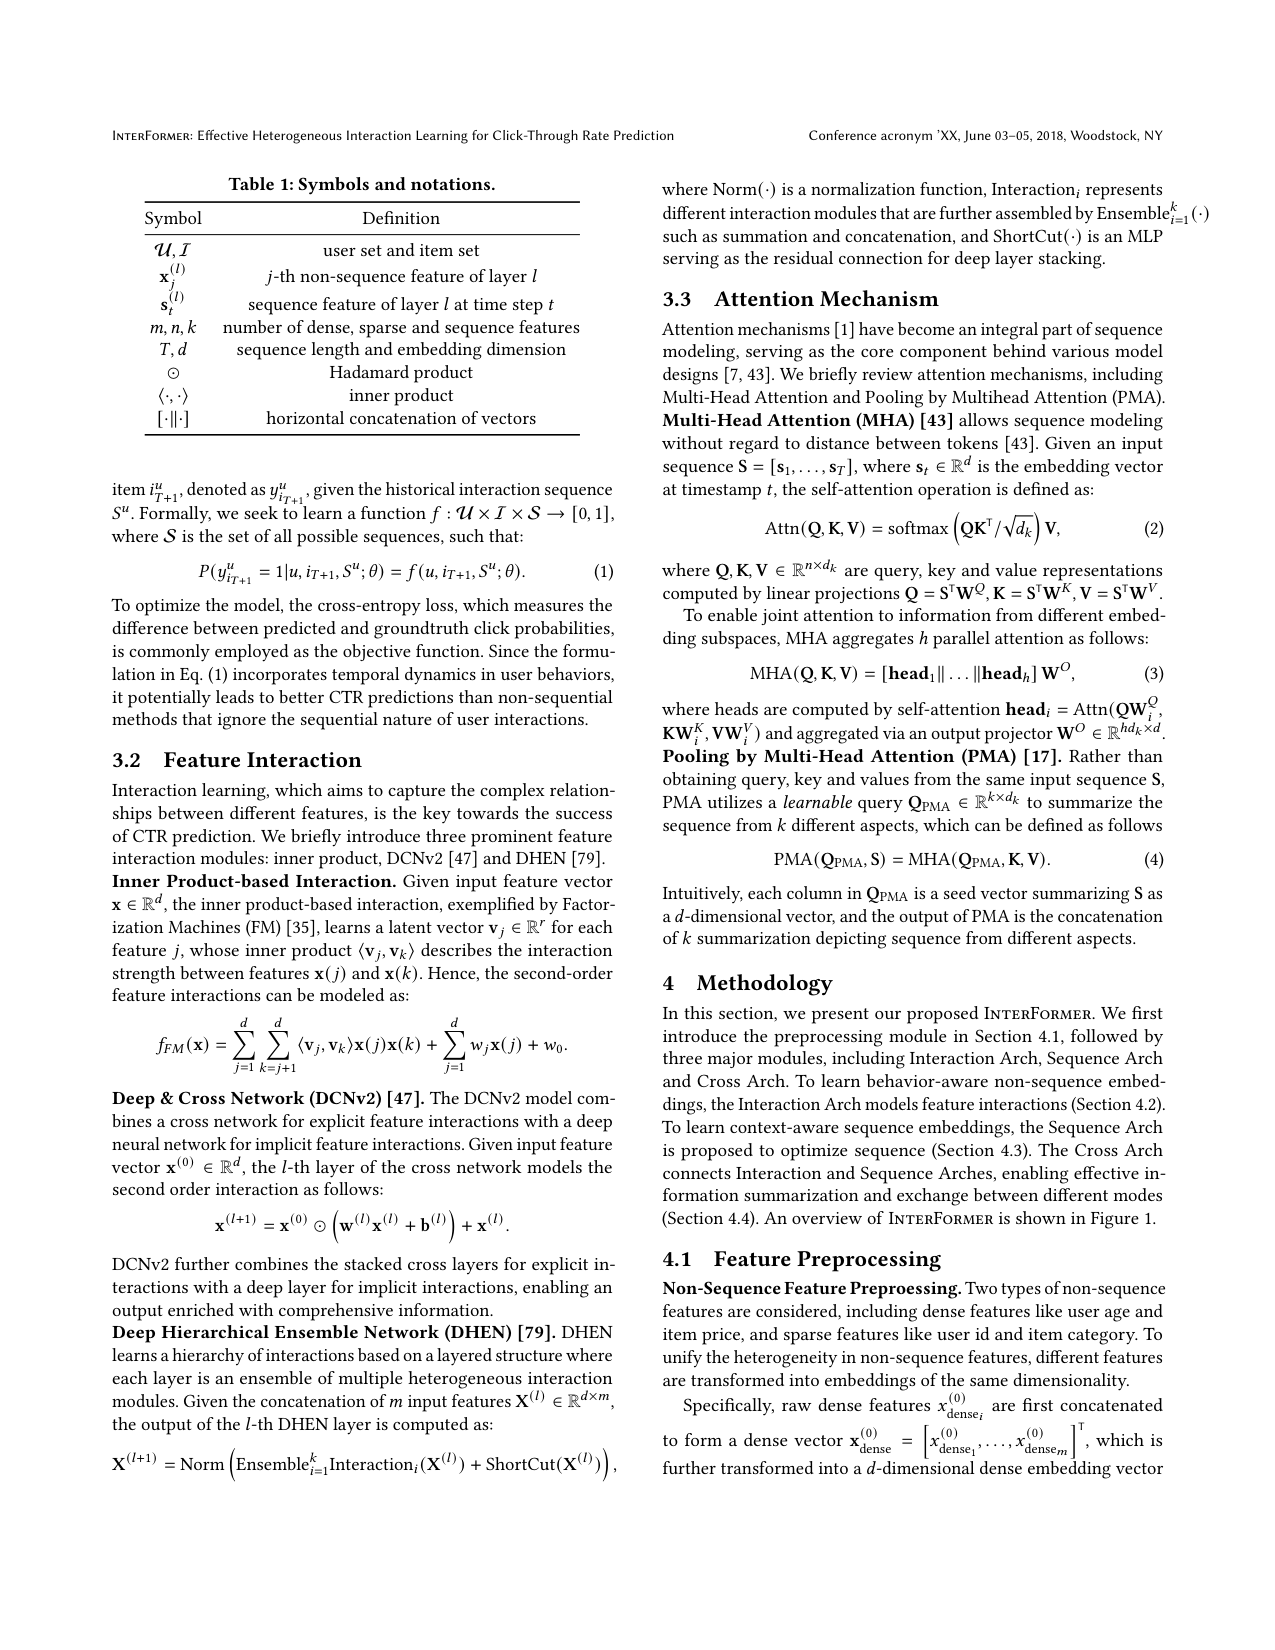
\includegraphics[width=\linewidth]{fig1_overview.png}
  \caption{An overview of the InterFormer model architecture (from the paper).}
\end{figure}

\subsection*{Challenges}
\begin{itemize}
  \item \textbf{Insufficient inter-mode interaction.} Prior heterogeneous CTR models often have \emph{unidirectional} information flow between non-sequential (profile/content) features and sequential (behavior) features, limiting ``mutual benefits'' across modes.
  \item \textbf{Aggressive information aggregation.} Many approaches summarize sequences early, which can cause \emph{excessive information loss} before sequence context can influence non-sequence interaction learning.
  \item \textbf{Noisy/multi-source sequences.} Real systems may have multiple behavior sequences (click, conversion, etc.) with noise and varying lengths; naïve fusion can degrade both effectiveness and efficiency.
\end{itemize}

\subsection*{Key Initiatives}
\begin{itemize}
  \item \textbf{Interleaving (bidirectional) heterogeneous interaction learning.} InterFormer is designed so that sequence and non-sequence representations are updated in a mutually conditioning way across layers.
  \item \textbf{Retain full-token representations per mode; summarize only for exchange.} Instead of early pooling, InterFormer keeps the dimensionalities of each mode through stacked layers and uses a \emph{separate Cross Arch} to selectively summarize information for cross-mode exchange.
  \item \textbf{Selective summarization via gating + multiple sequence summaries.} Non-sequence tokens are summarized with a gated selection; sequences are summarized with a combination of CLS tokens, PMA tokens, and recent tokens, then gated.
\end{itemize}

\subsection*{Methodology}
\begin{itemize}
  \item \textbf{Inputs / preprocessing.} Dense and sparse non-sequence features are embedded into a unified $d$-dim space. Each sequence event is embedded; multiple sequences can be unified/denoised using MaskNet-style self-masking.
  \item \textbf{Interaction Arch (behavior-aware non-seq interactions).} At each layer, a backbone interaction module (e.g., DOT/FM-like, DCNv2, DHEN) models interactions over the concatenation of non-seq tokens and a \emph{sequence summary} $S^{(\ell)}_{\mathrm{sum}}$, followed by an MLP shape-matching transform to preserve token-level mappings for stacking.
  \item \textbf{Sequence Arch (context-aware sequence modeling).} Sequence tokens are updated using (i) \emph{Personalized FFN (PFFN)} conditioned on a non-seq summary $X^{(\ell)}_{\mathrm{sum}}$, and (ii) \emph{Multi-Head Attention (MHA)} to capture long-range dependencies. The first layer prepends $X^{(1)}_{\mathrm{sum}}$ as a CLS token so attention can aggregate sequence info using non-seq context as query; rotary position embeddings are applied.
  \item \textbf{Cross Arch (selection + exchange).} To make exchange effective and efficient, the model computes low-dimensional summaries before exchanging:
  \begin{itemize}
    \item Non-seq summary: $X^{(\ell)}_{\mathrm{sum}} = \mathrm{Gating}(\mathrm{MLP}(X^{(\ell)}))$.
    \item Seq summary: $S^{(\ell)}_{\mathrm{sum}} = \mathrm{Gating}(S^{(\ell)}_{\mathrm{CLS}} \parallel S^{(\ell)}_{\mathrm{PMA}} \parallel S^{(\ell)}_{\mathrm{recent}})$.
  \end{itemize}
  \item \textbf{Design intent.} The authors emphasize separating ``information summarization'' from the two main arches to avoid aggressive aggregation while still enabling cross-mode interaction.
\end{itemize}

\subsection*{Experiments}
\begin{itemize}
  \item \textbf{Datasets.} Three public benchmarks: Amazon-Electronics (3.0M samples), TaobaoAd (25.0M), KuaiVideo (13.7M), plus an internal Meta dataset.
  \item \textbf{Baselines.} Non-seq: FM, xDeepFM, AutoInt+, DCNv2, FmFM, DOT, DHEN, Wukong. Seq: DIN, DIEN, BST, DMIN, DMR, TransAct.
  \item \textbf{Metrics.} AUC / gAUC, LogLoss; industrial: Normalized Entropy (NE) and system metrics (QPS, MFU).
  \item \textbf{Headline results (paper-quoted).} ``InterFormer achieves up to 0.14\% AUC improvement on benchmark datasets and 0.15\% Normalized Entropy (NE) gain on industrial dataset.''
  \item \textbf{Industrial scale (paper-quoted).} The internal dataset is described as ``containing 70B samples in total, hundreds of non-sequence features and 10 sequences of length 200 to 1,000.'' A 3-layer InterFormer reports ``a 0.15\% NE gain'' and ``24\% Queries Per Second (QPS) gain'' vs internal SOTA with similar FLOPs.
  \item \textbf{Ablations/analysis.} The paper tests (i) interleaving vs uni-directional/disabled flows, supporting the bidirectional benefit; (ii) selective aggregation vs average pooling/MLP/MHA early summarization; (iii) scaling with more sequence features and more layers.
\end{itemize}

\subsection*{References (selected)}
\begin{itemize}
  \item Transformer / attention for sequence modeling: Vaswani et al. (Transformer); DIN, DIEN; BST.
  \item Feature interaction baselines: FM; DCNv2; xDeepFM; AutoInt; DHEN; Wukong.
  \item Related industrial sequential CTR systems: TransAct; LiRank.
\end{itemize}

\noindent\textbf{arXiv:} \href{https://arxiv.org/abs/2411.09852}{2411.09852}

\end{document}
